% To see package versions
%\listfiles%

\documentclass{article}
\usepackage[utf8]{inputenc}
% for large margins
\usepackage[margin=1in]{geometry}
% for \verb
\usepackage{verbatim}
% for \verb inside lists
\usepackage[Q=yes]{examplep}

% fonts to remove the tilde
\usepackage[T1]{fontenc}
% \usepackage{beramono}

%for units
\usepackage[binary-units=true]{siunitx}

% to format the code
\usepackage[newfloat]{minted}
\usemintedstyle{borland}
% for code captioning
\usepackage{caption}

\newenvironment{code}{\captionsetup{type=listing}}{}
\SetupFloatingEnvironment{listing}{name=Code}


% to link to mimic
\usepackage{hyperref}

% to put graphs in
\usepackage{graphicx}
\graphicspath{ {images/} }
\usepackage{subcaption}


% bibliography
\usepackage[
backend=biber,
style=alphabetic,
sorting=ynt
]{biblatex}
\addbibresource{bib.bib}




\title{Benchmarking Parallel Application Performance Across SCD Infrastructure}
\author{Callum Iddon }
\date{March 2017}

\begin{document}

\definecolor{code-bg}{rgb}{0.95,0.95,0.95}
\setminted{bgcolor=code-bg}

\maketitle

\begin{abstract}
This is the abstract which is definitely TODO!
\end{abstract}


\tableofcontents

\section{Introduction}

    \subsection{Background}
        \paragraph{}
        The Scientific Computing Department (SCD) provides a number of compute resources. Across the different infrastructures, the varying CPUs, interconnect bandwidth and latencies have an unquantified effect on parallel applications. Also un-measured is the effect of choices within each service, such as using newer hardware or distributing cores between nodes.

    \subsection{In this project}
        \paragraph{}
        Comparison metrics are gathered for parallel application performance across three SCD services - SCARF, LOTUS and the SCD Cloud. The aim is to provide results that can inform deployment decisions for parallel applications using the message passing interface (MPI) libraries going forward.

        \paragraph{}
        Two specific metrics are recorded - bandwidth and latency - using the IMB PingPong benchmark. Application performance is then measured more generally according to the results from the HPL TOP500 test. On SCARF and LOTUS, these are taken on cores on the same node, spanning different nodes, and on different hardware versions. On the Cloud, they are taken from one VM and across two VMs (on different hypervisors).

    \subsection{Report Layout}
    TODO!

\section{Methods}

    \subsection{Overview}
    \label{overview-of-methods}
    There are two benchmarking applications to run on each system.

    \begin{description}
        \item[IMB PingPong] uses MPI to send messages of increasing size both ways between two processes \cite{intel2016}. Latency can be recorded as the average time for the message of zero size to cross one way between the two processes. Bandwidth can be recorded as the rate of throughput at different message sizes. The only dependency to run this benchmark is an MPI library.
        \item[HPL TOP500] solves a large matrix problem over distributed compute and memory resources \cite{hpl2016}. The time taken to solve the problem gives a measure of parallel application performance in flops (floating point operations per second). The software relies on a linear algebra library as well as an MPI library.
    \end{description}

    \subsection{Installation} \label{installation}

        \paragraph{}
        On the Cloud, the benchmarks need to be installed from scratch, alongside any dependencies. On SCARF and LOTUS, the MPI and linear algebra libraries are pre installed alongside HPL but IMB must be compiled from source and linked to the existing MPI libraries.

        \subsubsection{Cloud} \label{cloud-installation}

        \paragraph{}
        An SL6 no GUI virtual machine was used. The MPI library was OpenMPI and the linear algebra library was OpenBLAS (both from yum). A makefile was created to link to these libraries (Appendix \ref{appendix:makefile}).

            \begin{code}
            \captionof{listing}{Installing IMB and HPL on a Cloud VM}
            \label{code:builds-cloud-build-sh}
            \begin{minted}{bash}
# Install IMB PingPong
sudo yum -y install openmpi-devel  # install OpenMPI
wget https://software.intel.com/sites/default/files/managed/a3/53/IMB_2017.tgz
tar -xvf IMB_2017.tgz
source /etc/profile.d/modules.sh   # enable environment-modules
module load openmpi-1.10-x86_64    # load the MPI module
cd imb/imb/src
make all CC=mpicc                  # compile
cd -

# Install HPL
wget http://www.netlib.org/benchmark/hpl/hpl-2.2.tar.gz
tar -xvf hpl-2.2.tar.gz
sudo yum -y install openblas-devel openblas-static # install OpenBLAS
cd hpl-2.2/
# Copy in the makefile from the appendix now.
make arch=Linux_SL6_Intel64                        # compile
            \end{minted}
            \end{code}


        To run MPI between VMs on the Cloud (without a scheduler), SSH keys must be set up. There is no need for encryption provided the keys never leave either machine.
            \begin{code}
            \captionof{listing}{Setting up SSH keys between
            Cloud VMs}
            \label{code:builds-cloud-setupssh-sh}
            \begin{minted}{bash}
# On both VMs
sudo chown $USER:root ~/.ssh # Cloud VMs start with root:root, allow yourself access

# On one
ssh-keygen -t rsa # create key pair
cat ~/.ssh/id_rsa.pub >> ~/.ssh/authorized_keys # allow access to key
scp ~/.ssh/* <other VM hostname>:~/.ssh/ # copy this setup to the other machine
            \end{minted}
            \end{code}

        \subsubsection{SCARF and LOTUS}
        On both LOTUS and SCARF, the IMB PingPong benchmark was compiled from source.

            \begin{code}
            \captionof{listing}{Installing IMB on SCARF and LOTUS}
            \label{code:builds-jasmin_scarf-buildimb-sh}
            \begin{minted}{bash}
# Install IMB PingPong
wget https://software.intel.com/sites/default/files/managed/a3/53/IMB_2017.tgz
tar -xvf IMB_2017.tgz
cd imb/imb/src
gmake all CC=mpicc
            \end{minted}
            \end{code}


        On LOTUS, the HPL binary is located at \verb|/apps/src/hpl/hpl-2.2/bin/Linux_Intel64/xhpl| which is installed using the Intel MKL and Platform MPI libraries.

        On SCARF, HPL is optimised for each processor at \verb|/apps/procspec/hpl/2.2/bin/Linux_Intel64/xhpl|, to avoid this optimisation advantage, the SCARF10 (least optimised) version was used for all processors by copying this binary to a shared location between processors (see section \ref{running-HPL-SCARF}).




    \subsection{Running IMB PingPong}

        \paragraph{}
        In general, the benchmarks are submitted by shell scripts that take care of configuration parameters, platform specific parameters (eg LSF flags) and running repeats of the benchmarks. On the systems where there is a job scheduler (LOTUS and SCARF), these scripts submit the jobs where the benchmarks are actually run. On the Cloud, a cronjob is setup to run the script at regular intervals.

        \subsubsection{Configuration}

        \paragraph{}
        There is no configuration file required for the IMB benchmarks but a number of command line options are available.

        \begin{description}
            \item[iter n] ensures that \verb|n| repeats of each message size are taken and averaged. 1000 was chosen because it was the largest number of repeats that maintained a reasonable time to run on the slowest infrastructure (Cloud, between two VMs). It was also the default for smaller message sizes.
            \item[time t] sets a maximum time \verb|t|(s) for all repeats of a message size. 200 was chosen because it is significantly high such that this maximum was never reached.
            \item[msglog a:b] sets a minimum and maximum ($2^{a}$, $2^{b}$ respectively) for the message sizes.
            \item[iter\_policy] sets the behaviour with large message sizes and whether to reduce the number of repeats. Given that the number of repeats is feasible, setting this to \verb|off| means that the same number of repeats are tested for each message size.
        \end{description}

        \subsubsection{SCARF}
            \begin{enumerate}
                \item Create a top directory and \verb|cd| into it (e.g. \verb|/home/cseg/scarf565/SCARF_IMB|).
                \item Install IMB PingPong inside this directory as in Code \ref{code:builds-cloud-build-sh}. This should create \verb|imb/imb/src/IMB-MPI1|.
                \item Submit jobs to run the benchmark for five repeats across each host group. For each host group, run the benchmark between hosts using TCP, using Infiniband and on the same host. Use Code \ref{code:tests-scarf_imb-runimbscarf-sh} from inside the top directory.
                    \begin{code}
                    \captionof{listing}{Submitting IMB to SCARF}
                    \label{code:tests-scarf_imb-runimbscarf-sh}
                    \begin{minted}[breaklines=true]{bash}
#! /bin/bash
hostgroups=(scarf10 scarf11 scarf12 scarf13 scarf14 scarf15 scarf16)
# Make the outputs directory if it doesn't exist
mkdir -p $PWD/outputs
for specificHost in ${hostgroups[@]}; do # For each hostgroup
    for perTile in 1 2; do # Span one node or two
        if [ $perTile -eq 1 ]; then
            # If going between nodes, specify different interconnect flags
            pFlagOptions=(-TCP -IBV)
        else
            # If not, there are no interconnect flags
            pFlagOptions=("")
        fi
        for pFlag in "${pFlagOptions[@]}"; do # Step through interconnect flags
            for repeat in 1 2 3 4 5; do # Repeat the benchmark

bsub << %EndOfInput%
#BSUB -x
#BSUB -n 2
#BSUB -R "span[ptile=$perTile]"
#BSUB -J PingPong
#BSUB -o $PWD/outputs/%J.out
#BSUB -e $PWD/outputs/%J.err
#BSUB -W 0:45
#BSUB -m "$specificHost"
mpirun -lsf -prot $pFlag $PWD/imb/imb/src/IMB-MPI1 -iter 1000 -time 200 -msglog 0:24 -iter_policy off PingPong
%EndOfInput%

            done
        done
    done
done

                \end{minted}
                \end{code}
                \item This will create \verb|.err| and \verb|.out| files for each run of the benchmark under a directory \verb|outputs/|.
            \end{enumerate}
        \subsubsection{LOTUS}
            The method for running IMB PingPong on LOTUS is similar but there is no Infiniband available and there is a different \verb|mpirun| command.

            \begin{enumerate}
                \item Create a top directory and \verb|cd| into it (e.g. \verb|/home/users/ciddon/JASMIN_IMB|).
                \item Install IMB PingPong inside this directory as in Code \ref{code:builds-cloud-build-sh}. This should create \verb|imb/imb/src/IMB-MPI1|.
                \item Submit jobs to run the benchmark for 5 repeats across each host group. For each host group, run the benchmark between hosts and within the same host. Use Code \ref{code:tests-jasmin_hpl-runimbjasmin-sh} from inside the top directory.

                    \begin{code}
                    \captionof{listing}{Submitting IMB to LOTUS}
                    \label{code:tests-jasmin_hpl-runimbjasmin-sh}
                    \begin{minted}[breaklines=true]{bash}
#! /bin/bash
hostgroups=(ivybridge512G ivybridge2000G haswell256G ivybridge128G broadwell256G)
# Make the outputs directory if it doesn't exist
mkdir -p $PWD/outputs
for specificHost in ${hostgroups[@]}; do # For each hostgroup
    for perTile in 1 2; do # Span one or two nodes
        for repeat in 1 2 3 4 5; do # Repeat the benchmark

bsub << %EndOfInput%
#BSUB -x
#BSUB -q par-multi
#BSUB -n 2
#BSUB -R "span[ptile=$perTile]"
#BSUB -J PingPong
#BSUB -o $PWD/outputs/%J.out
#BSUB -e $PWD/outputs/%J.err
#BSUB -W 0:45
#BSUB -m "$specificHost"
mpirun.lotus -prot $PWD/imb/imb/src/IMB-MPI1 -iter 1000 -time 200 -msglog 0:24 -iter_policy off PingPong
%EndOfInput%

        done
    done
done
                    \end{minted}
                    \end{code}
                \item This creates the same \verb|.out| and \verb|.err| files as above.
            \end{enumerate}
        \subsubsection{Cloud}

            \paragraph{}
            Two virtual machines are required to run IMB PingPong. The main VM (where the job is initialised from) must have at least two cores. This allows running the benchmark between two VMs and on just the main VM without re-installation.

            \paragraph{}
            Using \url{http://mimic.gridpp.rl.ac.uk/}, under the \verb|Cloud -> Open Nebula| section, find the VMs and ensure that they are on different hypervisors (by clicking for more information).

            \begin{enumerate}
                \item Install IMB PingPong in the home directory of both VMs and setup SSH as in section \ref{cloud-installation}.
                \item Create a top directory on the main VM eg \verb|/home/tan49775/Cloud_IMB|.
                \item Create a script (Code \ref{code:tests-cloud_imb-runimbcloud-sh}) in this top directory which will run a repeat of the benchmark each time it is called, incrementing a count file to keep track of the number of repeats. The script ensures the benchmark is run 30 times within the same host and then 30 times between the two VMs. There is no 'exclusive' on the cloud so the average over a larger number of repeats ensures a better representation of typical use. Use a different \verb|HOME_DIR|, \verb|START_DIR| and host address.
                    \begin{code}
                    \captionof{listing}{The script to run IMB once on each call over cron}
                    \label{code:tests-cloud_imb-runimbcloud-sh}
                    \begin{minted}[breaklines=true]{bash}
#! /bin/bash

# Enable the module command
source /etc/profile.d/modules.sh
# Use the module command to set the mpi env
module load openmpi-1.10-x86_64

# Set up some variables
REPEATS_FOR_EACH=30
# Set HOME_DIR and START_DIR to the top directory
HOME_DIR=/home/tan49775  # should contain imb/imb/src.. and Cloud_IMB
START_DIR=$HOME_DIR/Cloud_IMB
COUNT=$START_DIR/count

# Make the output directory if needed
mkdir -p $START_DIR/outputs

num=$(date +"%Y%m%d_%H%M%S")
outputFile=$START_DIR/outputs/$num.out
errorFile=$START_DIR/outputs/$num.err

# If the count file does not exist then initialise it
if [ ! -s $COUNT ]; then echo "1" > $COUNT; fi

# If done enough repeats of one host and two hosts then exit
if [ $(cat $COUNT) -gt $((2 * $REPEATS_FOR_EACH)) ]; then exit 0; fi

# If done enough repeats for one host then use two hosts
if [ $(cat $COUNT) -gt $REPEATS_FOR_EACH ]; then
    echo "#HOSTS=2" > $outputFile
    # Edit the two host addresses here as necessary
    multiHostFlags="--prefix /usr/lib64/openmpi-1.10/ --map-by node  --rank-by node --host vm275.nubes.stfc.ac.uk,vm15.nubes.stfc.ac.uk"
else # Otherwise only use this host
    echo "#HOSTS=1" > $outputFile
    multiHostFlags=""
fi

# Run the benchmark
mpirun -np 2 $multiHostFlags $HOME_DIR/imb/imb/src/IMB-MPI1 -iter 1000 -msglog 0:24 -iter_policy off -time 200 PingPong 2> $errorFile >> $outputFile

# Increment the count file
echo $(($(cat $COUNT) + 1)) > $COUNT
                    \end{minted}
                    \end{code}
                \item Make the script executable using \mintinline{bash}{chmod 755 run_IMB_Cloud.sh}.
                \item Setup a crontab to run the script at 20 minute intervals.

                    \begin{minted}{bash}
05,25,45 * * * * /home/tan49775/Cloud_IMB/run_IMB_Cloud.sh
                    \end{minted}
                \item Again, similar output files are produced.
            \end{enumerate}

        \subsubsection{Interpreting Results}
            \paragraph{}
            The standard output from IMB PingPong is shown in Appendix \ref{appendix:imb-example-output}. As explained in Section \ref{overview-of-methods}, latency is recorded from the first entry in the \verb|t[usec]| column - where the message size is zero. Bandwidth is recorded from the \verb|Mbytes/sec| column. Different message sizes are of interest.
            TODO: NEATEN THIS UP





    \subsection{Running HPL}
        \paragraph{}
        Similarly to running IMB, shell scripts are used with cron or LSF for each setup to submit the necessary repeats and apply platform parameters. In the case of HPL, a configuration file is supplied.

        \subsubsection{Configuration}
            \paragraph{}
            HPL uses a configuration file to specify the problem size and the computational parameters (how to split the matrix and what functions to use). On execution, it looks in the working directory and reads from \verb|HPL.dat|. The full file used is included in Appendix \ref{appendix:hpl-conf}.


            \paragraph{}
            The first parameter to choose is the number of cores to use when running the benchmark. The same number should be chosen for LOTUS, SCARF and the Cloud to allow comparison. Given that the Cloud has a limit of 5 cores per user (split across as many VMs) that specifies an upper bound. The parameters \verb|P| and \verb|Q| should be approximately equal and \verb|P| multiplied by \verb|Q| is the number of processors. In order to avoid \verb|P| or \verb|Q| being 1, 2 was chosen for both values giving a total of 4 cores. To balance across hosts, measurements were taken with four cores from the same node and with two cores on each node.

            \paragraph{}
            Some initial tests were done across the infrastructures to choose a value of \verb|NB| (the block size) that was reasonably well performing with respect to other values in the default interval [32, 256]. However, care was taken to avoid tuning this value to a particular system and these initial test were only to confirm that it was not a radically poor choice for any setup. 180 was used.

            \paragraph{}
            The main parameter is 'problem size' (\verb|N|)  which is the side length of the matrix to be solved. According to \cite{hpl2016}, the largest size that will fit in memory is recommended. The Cloud limits users to 20GB of memory so this was used as an upper bound. Each element in the matrix is a double precision float (8 bytes). This means that a total of $2.5 \times 10 ^ 9$ elements can be used. Using the recommend 80\% figure (to leave room for the OS), this gives a side length of around 44721. It is also beneficial to have a multiple of NB so 44640 was chosen.

            \paragraph{}
            Provided the same file is used for each test (to an extent) the content of this file is insignificant - it will still provide a comparison of parallel application performance. Where possible, advice in the "FAQ" and "tuning" sections of \cite{hpl2016} was followed, using default or suggested values to attempt to remain neutral. Of course, it would be possible to tune this configuration file for each setup and achieve some faster speeds but this would likely be at the expense of other setups and introduce a bias. Any case where there was no default value given is justified above.



        \subsubsection{SCARF}
        \label{running-HPL-SCARF}
        \begin{enumerate}
            \item Create a top directory (e.g. \verb|/home/cseg/scarf656/SCARF_HPL|) and \verb|cd| into it.
            \item Run \mintinline{bash}{bsub -m scarf10 "cp /apps/procspec/hpl/2.2/bin/Linux_Intel64/xhpl ."} to copy the SCARF10 precompiled HPL binary into this directory.
            \item Copy in \verb|HPL.dat| from Appendix \ref{appendix:hpl-conf}.
            \item Submit jobs to run the benchmark for five repeats across each host group. For each host group, run the benchmark between two hosts using TCP and using Infiniband; and on the same host. Use Code \ref{code:tests-scarf_hpl-runhplscarf-sh} from inside the top directory.


            \begin{code}
            \captionof{listing}{Submitting HPL to SCARF}
            \label{code:tests-scarf_hpl-runhplscarf-sh}

            \begin{minted}{bash}
#! /bin/bash
hostgroups=(scarf10 scarf11 scarf12 scarf13 scarf14 scarf15 scarf16)
# Make the outputs directory if it doesn't exist
mkdir -p $PWD/outputs
for specificHost in ${hostgroups[@]}; do # For each hostgroup
    for perTile in 2 4; do # Span one node or two
        if [ $perTile -eq 2 ]; then
            # If going between nodes, specify different interconnect flags
            pFlagOptions=(-TCP -IBV)
        else
            # If not, there are no interconnect flags
            pFlagOptions=("")
        fi
	    for pFlag in "${pFlagOptions[@]}"; do # Step through interconnect flags
            for repeat in 1 2 3 4 5; do # repeat the benchmark

bsub << %EndOfInput%
#BSUB -x
#BSUB -n 4
#BSUB -R "span[ptile=$perTile]"
#BSUB -J HPL
#BSUB -o $PWD/outputs/%J.out
#BSUB -e $PWD/outputs/%J.err
#BSUB -W 1:00
#BSUB -m "$specificHost"
module load intel/15.3
module load intel/mkl/11.3.1.150
mpirun -lsf -prot $pFlag $PWD/xhpl
%EndOfInput%

            done
        done
    done
done
            \end{minted}
            \end{code}
            \item Output and error files are placed into a sub-directory \verb|outputs| for analysis.
        \end{enumerate}


        \subsubsection{LOTUS}

        \paragraph{}
        HPL requires a linear algebra library to run. On SCARF and LOTUS, this in Intel's MKL. The environment for this is set up using the \mintinline{bash}{module load} command and on SCARF, this is passed to the other process using system daemons. On LOTUS, MPI is configured to run over SSH meaning that each new process has a different environment. For this reason, it is necessary to pass the \verb|LD_LIBRARY_PATH| environment variable in the \mintinline{bash}{mpirun.lotus} command (see Code \ref{code:tests-jasmin_hpl-runhpljasmin-sh}).

        \begin{enumerate}

            \item Create a top directory (e.g. \verb|/home/users/ciddon/JASMIN_HPL|) and \verb|cd| into it.

            \item Copy in \verb|HPL.dat| from Appendix \ref{appendix:hpl-conf}.

            \item Submit jobs to run the benchmark for five repeats across each host group. For each host group, run the benchmark between two hosts and on the same host. Use Code \ref{code:tests-jasmin_hpl-runhpljasmin-sh} from inside the top directory.

            \begin{code}
            \captionof{listing}{Submitting HPL to LOTUS}
            \label{code:tests-jasmin_hpl-runhpljasmin-sh}

            \begin{minted}[breaklines=true]{bash}
#! /bin/bash
hostgroups=(ivybridge512G ivybridge2000G haswell256G ivybridge128G broadwell256G)
# Make the outputs directory if it doesn't exist
mkdir -p $PWD/outputs
for specificHost in ${hostgroups[@]}; do # For each hostgroup
    for perTile in 2 4; do # Span one (4) or two (2) nodes
        for repeat in 1 2 3 4 5; do # Repeat the benchmark

bsub << %EndOfInput%
#BSUB -x
#BSUB -q par-multi
#BSUB -n 4
#BSUB -R "span[ptile=$perTile]"
#BSUB -J HPL
#BSUB -o $PWD/outputs/%J.out
#BSUB -e $PWD/outputs/%J.err
#BSUB -W 1:00
#BSUB -m "$specificHost"
. /etc/profile.modules
module load intel/15.1
module load intel/mkl/11.3.1.150
mpirun.lotus -e LD_LIBRARY_PATH=\$LD_LIBRARY_PATH -prot /apps/src/hpl/hpl-2.2/bin/Linux_Intel64/xhpl
%EndOfInput%

        done
    done
done
            \end{minted}
            \end{code}
            \item Output and error files are placed into a sub-directory \verb|outputs| for analysis.
        \end{enumerate}



        \subsubsection{Cloud}

            \paragraph{}
            The Cloud limits total memory per user to 20GB. All this is required for each test so run them over two VMs (2CPUs and 10GB RAM each) and then install a single VM (4 CPUs and 20GB RAM) to run the individual tests.

            \paragraph{}
            Use \url{http://mimic.gridpp.rl.ac.uk/} to as described for running IMB to check that then VMs are on different hypervisors.

            \begin{enumerate}
                \item \label{item:cloud-hpl-repeat-start} Install HPL in the home direction of both VMs using \ref{code:builds-cloud-build-sh}

                \item Create a top directory under the main VM eg \verb|/home/tan49775/Cloud_HPL|.

                \item Copy in the \verb|HPL.dat| from Appendix \ref{appendix:hpl-conf}.

                \item Create a script (Code \ref{code:tests-cloud_hpl-runhplcloud-sh}) in the top directory which will run a repeat of the benchmark two nodes each time it is called for 30 repeats. A larger number of repeats is used because of the lack of exclusive jobs on the cloud - more results to average. Code \ref{code:tests-cloud_hpl-runhplcloud-sh} only runs the benchmark over two nodes. Use different \verb|HOME_DIR|, \verb|START_DIR| and host addresses.

                    \begin{code}
                    \captionof{listing}{The script to run HPL once on each call over cron over two nodes}
                    \label{code:tests-cloud_hpl-runhplcloud-sh}
                    \begin{minted}[breaklines=true]{bash}
#! /bin/bash

source /etc/profile.d/modules.sh
module load openmpi-1.10-x86_64

REPEATS=30
HOME_DIR=/home/tan49775  # should contain hpl-2.2 and Cloud_HPL
START_DIR=$HOME_DIR/Cloud_HPL
COUNT=$START_DIR/count


# Make the output directory if needed
mkdir -p $START_DIR/outputs
cd $START_DIR

num=$(date +"%Y%m%d_%H%M%S")
outputFile=$START_DIR/outputs/$num.out
errorFile=$START_DIR/outputs/$num.err

# If the count file does not exist then initialise it
if [ ! -s $COUNT ]; then echo "1" > $COUNT; fi

# If done enough repeats then exit
if [ $(cat $COUNT) -gt $REPEATS ]; then exit 0; fi


# Run the benchmark
mpirun -np 4 --prefix /usr/lib64/openmpi-1.10/ --map-by node  --rank-by node --host vm275.nubes.stfc.ac.uk,vm15.nubes.stfc.ac.uk $HOME_DIR/hpl-2.2/bin/Linux_SL6_Intel64/xhpl 2> $errorFile >> $outputFile

# Increment the count file
echo $(($(cat $COUNT) + 1)) > $COUNT
                    \end{minted}
                    \end{code}

                \item Make the script executable using \mintinline{bash}{chmod 755 run_HPL_Cloud_2Nodes.sh}.
                \item \label{item:cloud-hpl-repeat-end} Setup a crontab to run the script at 50 minute intervals.

                    \begin{minted}{bash}
50 * * * * /home/tan49775/Cloud_HPL/run_HPL_Cloud_2Nodes.sh
                    \end{minted}
                \item Copy the output files to a safe place and reinstall the machine as a single VM with 4CPUs and 20GB of RAM.

                \item Repeat steps \ref{item:cloud-hpl-repeat-start} to \ref{item:cloud-hpl-repeat-end} above, removing the flags causing it to run over two nodes.

                \begin{minted}[breaklines=true]{bash}
--prefix /usr/lib64/openmpi-1.10/ --map-by node  --rank-by node --host vm275.nubes.stfc.ac.uk,vm15.nubes.stfc.ac.uk
                \end{minted}

            \end{enumerate}


        \subsubsection{Interpreting Results}
            Appendix \ref{appendix:hpl-example-output} contains an example output from one run of HPL. The result of this benchmark is the final value for 'Gflops' (3.297e+01 in this case).


\section{Results}
    \paragraph{} The individual output files for each run were saved and the useful pieces of data were parsed for analysis. This section presents the results and explains the additional experiments to improve and update the results.

    \paragraph{}
    The busy queues on LOTUS forced submitting some of the benchmarks with different 'BSUB' parameters to the methods section. For all jobs on 'ivybridge2000G' and 3 HPL on 'ivybridge512G' over two hosts, the jobs were waiting for weeks without being run. Instead, a host reservation was used - removing the \mintinline{bash}{-m} parameter and adding a \mintinline{bash}{-U}. The different BSUB parameters should have had no effect on the results as they only define how the job is sumbitted rather than how they are run.

    \subsection{IMB PingPong}

        \subsubsection{SHM first look and adapted experiment}
            \begin{figure}[ht]
                \centering
                \begin{subfigure}{.5\textwidth}
                  \centering
                  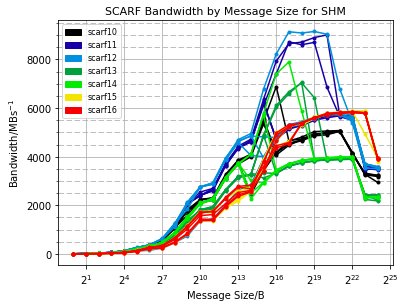
\includegraphics[width=\textwidth]{scarf_bandwidth-msgsize_shm}
                  \caption{SCARF}
                \end{subfigure}%
                \begin{subfigure}{.5\textwidth}
                  \centering
                  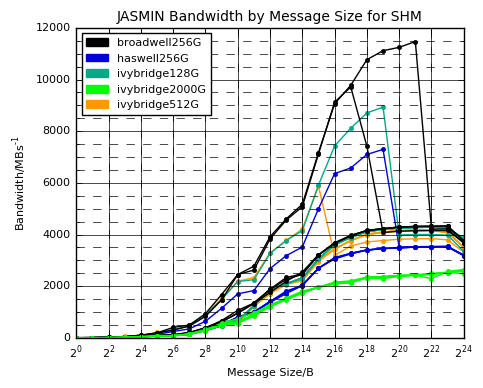
\includegraphics[width=\textwidth]{jasmin_bandwidth-msgsize_shm}
                  \caption{LOTUS}
                \end{subfigure}
            \caption{Before specifying CPUs}
            \label{figure:imb-before-cpus}
            \end{figure}

            \paragraph{}
            Figure \ref{figure:imb-before-cpus} shows the initial results for IMB over SCARF and LOTUS and shared host memory (SHM - between cores on the same host). Each colour represents a different host group (same hardware) and each line is an individual repeat. For each host group, there seems to be two distinct paths rather than one. For example, scarf11 has a bandwidth of roughly \SI{8300}{\mega\byte\per\second} for two repeats but roughly \SI{5200}{\mega\byte\per\second} for the other three at $2^{18}$\si{\byte}. Occasionally (as seen in scarf14) a repeat will begin on the higher path and drop down to the lower (at $2^{17}$ \si{\byte}).

            \paragraph{}
            A likely explanation is the multiple physical CPUs included in each host. Each host has two or more but the job is submitted without specifying the mapping. The random allocation would create the distinct paths. Without mapping, it may be possible for a job to move from one CPU to two CPUs or vice versa which would lead to the switching behavior in Figure \ref{imb-before-cpus}.

            \paragraph{}
            To eliminate this variation and to test if this is actually the cause, the tests were repeated over SHM for SCARF and LOTUS, specifically mapping to one or two CPUs. For one CPU, \mintinline{bash}{numactl --cpunodebind=0 --} was passed as a command line option to the respective \mintinline{bash}{mpirun} command. \mintinline{bash}{-cpu_bind=MAP_CPU:0,15} was used for two. If this is the cause of the variation, the new results should exhibit the same distinction but have a unique path for each mapping. The CPU mapping should remove the jumping between paths.

            \paragraph{}
            Figure \ref{figure:imb-after-cpus} shows the new results. Similar distinctions between paths to Figure \ref{figure:imb-before-cpus} are shown to be grouped by the CPU mapping (shown in the key).

            \begin{figure}[ht]
                \centering
                \begin{subfigure}{.5\textwidth}
                  \centering
                  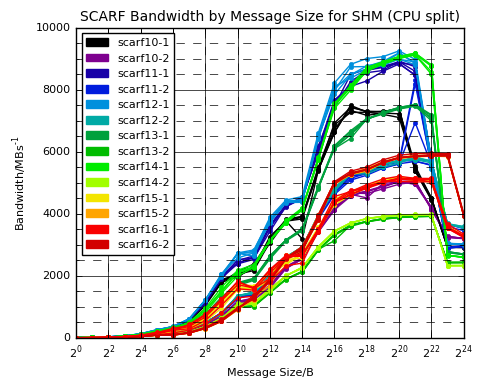
\includegraphics[width=\textwidth]{scarf_bandwidth-msgsize_shm_split}
                  \caption{SCARF}
                \end{subfigure}%
                \begin{subfigure}{.5\textwidth}
                  \centering
                  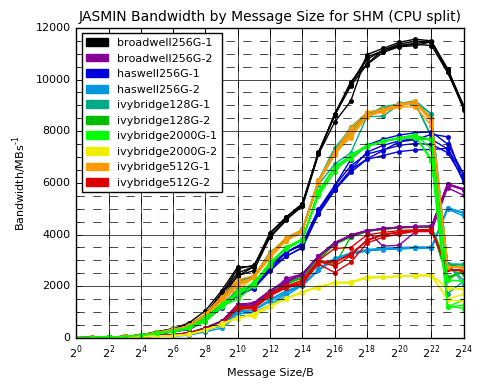
\includegraphics[width=\textwidth]{jasmin_bandwidth-msgsize_shm_split}
                  \caption{LOTUS}
                \end{subfigure}
            \caption{After specifying CPU mapping}
            \label{figure:imb-after-cpus}
            \end{figure}


    \subsection{HPL}

\section{Evaluation}

\section{Conclusion}





















\printbibliography[title={Sources}]






































\appendix
    \section*{Appendices}
    \addcontentsline{toc}{section}{Appendices}
    \renewcommand{\thesubsection}{\Alph{subsection}}

    \subsection{HPL SL6 Makefile}
    \label{appendix:makefile}

    \paragraph{}
    This make file is used to link the HPL binary to the libraries it requires. The comments are removed for clarity but the format follows the example in the \verb|hpl-2.2.tar| archive \verb|hpl-2.2/setup/Make.Linux_Intel64|. It should be saved as \verb|hpl-2.2/Make.Linux_SL6_Intel64|.
        \begin{code}
        \captionof{listing}{The HPL SL6 Makefile}
        \label{code:builds-cloud-make-linux_sl6_intel64}
        \begin{minted}{make}
SHELL        = /bin/sh
CD           = cd
CP           = cp
LN_S         = ln -fs
MKDIR        = mkdir -p
RM           = /bin/rm -f
TOUCH        = touch
ARCH         = Linux_SL6_Intel64
TOPdir       = $(HOME)/hpl-2.2
INCdir       = $(TOPdir)/include
BINdir       = $(TOPdir)/bin/$(ARCH)
LIBdir       = $(TOPdir)/lib/$(ARCH)
HPLlib       = $(LIBdir)/libhpl.a
MPdir        = /usr
MPinc        = -I$(MPdir)/include/openmpi-1.10-x86_64
MPlib        = $(MPdir)/lib64/openmpi-1.10/lib/libmpi.so
LAinc        =  /usr/include/openblas/
LAlib        =  /usr/lib64/libopenblas.so
F2CDEFS      = -DAdd__ -DF77_INTEGER=int -DStringSunStyle
HPL_INCLUDES = -I$(INCdir) -I$(INCdir)/$(ARCH) -I$(LAinc) $(MPinc)
HPL_LIBS     = $(HPLlib) $(LAlib) $(MPlib)
HPL_OPTS     = -DHPL_DETAILED_TIMING -DHPL_PROGRESS_REPORT
HPL_DEFS     = $(F2CDEFS) $(HPL_OPTS) $(HPL_INCLUDES)
CC           = mpicc
CCNOOPT      = $(HPL_DEFS)
OMP_DEFS     = -openmp
CCFLAGS      = $(HPL_DEFS) -O3 -w -z noexecstack -z relro -z now -Wall
LINKER       = $(CC)
LINKFLAGS    = $(CCFLAGS) $(OMP_DEFS) -mt_mpi
ARCHIVER     = ar
ARFLAGS      = r
RANLIB       = echo

        \end{minted}
        \end{code}

    \subsection{IMB Example Output}
        \label{appendix:imb-example-output}

        \paragraph{}
        The following is a section of the output from the IMB PingPong benchmark. The general information (e.g. start time) has been removed from the header, leaving just the output.
        \begin{minted}{text}
#---------------------------------------------------
# Benchmarking PingPong
# #processes = 2
#---------------------------------------------------
       #bytes #repetitions      t[usec]   Mbytes/sec
            0         1000         0.24         0.00
            1         1000         0.31         3.03
            2         1000         0.33         5.73
            4         1000         0.32        12.02
            8         1000         0.33        23.29
           16         1000         0.36        42.87
           32         1000         0.32        95.24
           64         1000         0.34       177.65
          128         1000         0.38       322.93
          256         1000         0.47       524.46
          512         1000         0.57       853.69
         1024         1000         0.73      1334.20
         2048         1000         1.02      1916.71
         4096         1000         2.00      1957.00
         8192         1000         2.97      2629.12
        16384         1000         5.06      3086.37
        32768         1000         8.39      3723.58
        65536         1000        13.45      4648.40
       131072         1000        23.42      5338.11
       262144         1000        40.61      6155.58
       524288         1000        72.47      6899.88
      1048576         1000       134.10      7456.95
      2097152         1000       262.16      7628.87
      4194304         1000       614.76      6506.58
      8388608         1000      1714.74      4665.43
     16777216         1000      3617.98      4422.35
        \end{minted}

    \subsection{HPL Configuration File}
        \label{appendix:hpl-conf}

        \paragraph{}
        The configuration file that was used with every HPL test is given below.

        \begin{minted}{text}
The HPL Configuration File for comparing LOTUS, SCARF
and the Cloud in SCD.
not_used     output file name (if any)
6            device out (6=stdout,7=stderr,file)
1            # of problems sizes (N)
44640        Ns
1            # of NBs
180          NBs
0            PMAP process mapping (0=Row-,1=Column-major)
1            # of process grids (P x Q)
2            Ps
2            Qs
16.0         threshold
1            # of panel fact
1            PFACTs (0=left, 1=Crout, 2=Right)
1            # of recursive stopping criterium
4            NBMINs (>= 1)
1            # of panels in recursion
2            NDIVs
1            # of recursive panel fact.
2            RFACTs (0=left, 1=Crout, 2=Right)
1            # of broadcast
1            BCASTs (0=1rg,1=1rM,2=2rg,3=2rM,4=Lng,5=LnM)
1            # of lookahead depth
1            DEPTHs (>=0)
2            SWAP (0=bin-exch,1=long,2=mix)
180          swapping threshold
0            L1 in (0=transposed,1=no-transposed) form
0            U  in (0=transposed,1=no-transposed) form
1            Equilibration (0=no,1=yes)
8            memory alignment in double (> 0)

        \end{minted}


    \subsection{HPL Example Output}
        \label{appendix:hpl-example-output}

        \paragraph{}
        The following is the output from a run of the HPL Benchmark. The description of the parameters has been truncated as well as the intermediate results.

        \begin{minted}{text}
================================================================================
HPLinpack 2.2  --  High-Performance Linpack benchmark  --   February 24, 2016
Written by A. Petitet and R. Clint Whaley,  Innovative Computing Laboratory, UTK
Modified by Piotr Luszczek, Innovative Computing Laboratory, UTK
Modified by Julien Langou, University of Colorado Denver
================================================================================
...
--------------------------------------------------------------------------------

- The matrix A is randomly generated for each test.
- The following scaled residual check will be computed:
      ||Ax-b||_oo / ( eps * ( || x ||_oo * || A ||_oo + || b ||_oo ) * N )
- The relative machine precision (eps) is taken to be               1.110223e-16
- Computational tests pass if scaled residuals are less than                16.0

Column=000000180 Fraction= 0.4% Gflops=5.839e+03
Column=000000360 Fraction= 0.8% Gflops=6.953e+01
Column=000000540 Fraction= 1.2% Gflops=5.027e+01
...
Column=000044460 Fraction=99.6% Gflops=3.297e+01
================================================================================
T/V                N    NB     P     Q               Time                 Gflops
--------------------------------------------------------------------------------
WR11R2C4       44640   180     2     2            1799.04              3.297e+01
HPL_pdgesv() start time Sun Mar 26 23:50:20 2017

HPL_pdgesv() end time   Mon Mar 27 00:20:19 2017

--VVV--VVV--VVV--VVV--VVV--VVV--VVV--VVV--VVV--VVV--VVV--VVV--VVV--VVV--VVV-
Max aggregated wall time rfact . . . :               6.76
+ Max aggregated wall time pfact . . :               1.22
+ Max aggregated wall time mxswp . . :               0.62
Max aggregated wall time update  . . :            1792.06
+ Max aggregated wall time laswp . . :              49.64
Max aggregated wall time up tr sv  . :               0.36
--------------------------------------------------------------------------------
||Ax-b||_oo/(eps*(||A||_oo*||x||_oo+||b||_oo)*N)=        0.0006845 ...... PASSED
================================================================================

Finished      1 tests with the following results:
              1 tests completed and passed residual checks,
              0 tests completed and failed residual checks,
              0 tests skipped because of illegal input values.
--------------------------------------------------------------------------------

End of Tests.
================================================================================

        \end{minted}

\end{document}
